\section{Experiments}

\subsection{Experimental setup}\label{sec:experiments:setup}

\paragraph{Simulation and robot}
The policies are trained in the IsaacGym~\citep{makoviychuk2021isaac} simulator using massively parallel environments.
The full policy learning pipeline can be trained on a single NVIDIA RTX 4090 GPU in less than 20 hours.
After training in simulation, the controller is directly deployed on a real Solo-12 quadruped robot.
The policy runs at $50 Hz$ on a Raspberry Pi 5.
Target joint positions are sent to the onboard PD controller running at $10 kHz$.
We use an Intel RealSense D-405 stereo camera to capture depth images and process them to resolution $48 \times 48$.
While the depth images are rendered every $5$ environment steps in simulation (i.e. $10$Hz in the time reference of the simulation), we provide the images at the speed of the depth pipeline on the real robot at $30Hz$.

When standing, the height of Solo is $26$cm and its body length is $45$cm, which is similar to the Unitree Go-1 used in~\citep{zhuang2023robot, cheng2023parkour}.
However, Go-1 has a thrust-to-weight ratio $2$ to $3$ times superior to Solo.
Thus, we don't expect to overcome obstacles as challenging as~\citep{zhuang2023robot, cheng2023parkour}.

\paragraph{Baselines and ablations}
We validate our approach in simulation and compare SoloParkour to the following baselines and ablations.
\begin{itemize}[topsep=-4pt,itemsep=1pt,partopsep=0pt, parsep=0pt]
    \item DAgger~\citep{ross2011reduction}: the method used in~\citep{cheng2023parkour, zhuang2023robot, agarwal2023legged} to distill the privileged policy into the visual policy using imitation learning through action relabelling with the privileged policy.
    \item Behavior Cloning (BC): distilling the privileged policy by training the visual policy directly with supervised learning on the privileged experience $\mathcal{D}_\text{priv}$.
    \item Privileged Reconstruction: training the vision module to reconstruct the privileged information from the history of depth and proprioceptive inputs, then reemploy the Stage 1 policy based on these reconstructions, aimed to resemble~\cite{agarwal2023legged, duan2023learning}.
    \item From Scratch: an ablation of our approach where we train the visual policy with RL from scratch, without privileged experience $\mathcal{D}_\text{priv}$.
    \item No Priv. Critic: an ablation of our approach where the critic of Stage 2 observes histories of depth images instead of the simplified privileged information.
    \item Visual RL w/o CaT: an ablation of our approach where we train the visual RL policy without constraints (but from experience from the same constrained Stage 1 policy).
\end{itemize}
We first train a privileged policy from Stage 1.
Then, except for BC which is much faster to train as it doesn't require querying the simulator, we train all these baselines and ablations with the same computational budget.
Finally, we compare their performance by executing the learned policies in simulation and measuring the distance traveled in the terrains of Figure~\ref{fig:terrains}.

%=================================================================================

\subsection{Simulation Experiments}



\begin{figure}[ht]
    \centering
    \begin{subfigure}[b]{\textwidth}
        \centering
        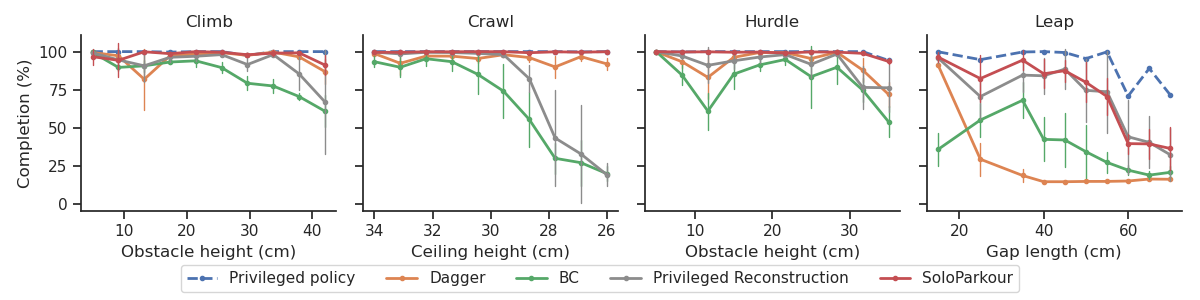
\includegraphics[width=\textwidth]{Assets/Results/completion_main.png}
        \caption{Comparison between SoloParkour and imitation-based distillation methods.}
        \label{fig:completion_main}
    \end{subfigure}

    \begin{subfigure}[b]{\textwidth}
        \centering
        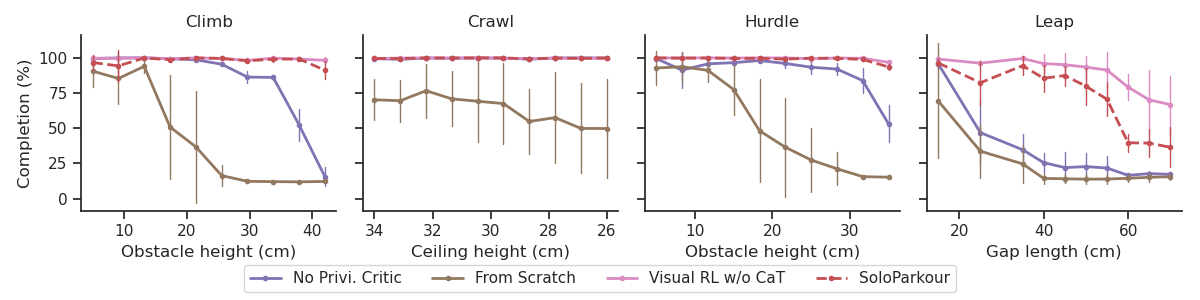
\includegraphics[width=\textwidth]{Assets/Results/completion_abla.png}
        \caption{Ablations of the proposed methods.}
        \label{fig:completion_abla}
    \end{subfigure}
    
    %\caption{Comparison of simulation results.}
    \caption{Average terrain completion (over 4 training seeds) by obstacle dimension for each policy.}
    \label{fig:completion_results}
    \vspace{-0.5cm}
\end{figure}

\paragraph{Comparison to supervised distillation}%Imitation-based
In Figure~\ref{fig:completion_main}, we compare SoloParkour against DAgger, BC and \textit{Privileged Reconstruction}.
For comparison, we also report the performances of the privileged policy used to train these methods.
SoloParkour performs roughly as well as the privileged policy on the hurdle, step, and crawl tracks and marginally worse on the leap track.
It outperforms the supervised distillation baselines on all terrains and at almost all levels of difficulty.
The difference is particularly significant against DAgger and BC on the leap terrains, where the robot must perform a complex motion to overcome the gaps, requiring perfect timing to succeed.
On these terrains, DAgger and BC often fail to propel themselves enough and miss the edge of the landing side of the platform, or ignore the gap and fall into it.
Meanwhile, \textit{Privileged Reconstruction} struggles on the crawl and climb terrains, where occlusions hinder accurate reconstruction of the surrounding terrain geometry.
We attribute these differences to our end-to-end training from pixels with the RL objective, which results in tighter coordination between vision and control, understood as a local action-perception refinement.


\paragraph{Ablative analysis}
In Figure~\ref{fig:completion_abla}, we examine the importance of two design choices for SoloParkour given the same computation budget.
Training the visual policy from scratch without privileged experience (\textit{from Scratch}) is much less sample-efficient and achieves poor performances overall, validating the importance of transferring privileged experience from the Stage 1 policy.
Having the critics process the full-depth observation instead of only the privileged information (\textit{No Priv. Critic}) causes additional computation overheads during Q-learning, which are yet unnecessary to train good visual policies in our setting.
As a result, given the same computation budget, \textit{No Priv. Critic} processes fewer samples and achieves lower performances than the full SoloParkour method. 


\paragraph{Constraints satisfaction}

%=================================================================================
\begin{wraptable}{r}{0.36\textwidth} 
    \vspace{-0.5cm}
    \centering
    \begin{tabular}{c|c|c|c}
        \toprule
        Step & Leap & Crawl & Average\\
        \midrule
        85\% & 70\% & 100\% & 85\% \\
        \bottomrule
    \end{tabular}
    \caption{Success rates achieved by the policies for different obstacles on the real robot, averaged over 2 training seeds and 10 trials per obstacle per seed.}
    \label{table:results}
\end{wraptable}

In Figure~\ref{fig:torque_comparison}, we examine the violation of the torque constraint for the front left shoulder joint and the base orientation constraint, as outlined in (\ref{eq:cstr_torque}).
We focused exclusively on successful trajectories where the robot managed to navigate the entire level in order to exclude data from extreme states, such as when the robot is falling outside of the track or gets endlessly stuck on a high obstacle.
Hence, we report results for only two gap lengths on the leap track for DAgger, as it fails to overcome larger gaps.
Thanks to off-policy CaT, SoloParkour maintains constraint compliance effectively after visuomotor RL, with torque violations under 4\% and base orientation violations under 10\% on most levels, despite the highly dynamic skills involved to overcome the obstacles.
These results are comparable to those of the privileged policy and supervised distillation baselines. 
By contrast, \textit{Visual RL w/o CaT} achieves higher terrain completion rates but at the cost of significantly increased constraint violations, rendering the policies unsuitable for real-world robot transfer.
Additional results on the satisfaction of a broader set of constraints are discussed in Appendix \ref{appendix:additional_results}.

\subsection{Real-Robot Experiments}

We deploy SoloParkour directly on the real Solo-12 and evaluate it to traverse challenging obstacles that involve climbing, crawling, and leaping (see Figure~\ref{fig:teaser}).
We found that the policy handled the depth vision signals sent by the camera, responding synchronously to obstacles at the right time.
Table \ref{table:results} reports the results achieved by SoloParkour.
Our approach successfully climbs a $40$cm step (1.5 times the robot's height), leaps over a $35$cm gap (78\% of its length), and crawls under obstacles $20$cm above the ground with high repeatability.




\begin{figure}[t]
    \centering
    \begin{subfigure}[b]{\textwidth}
        \centering
        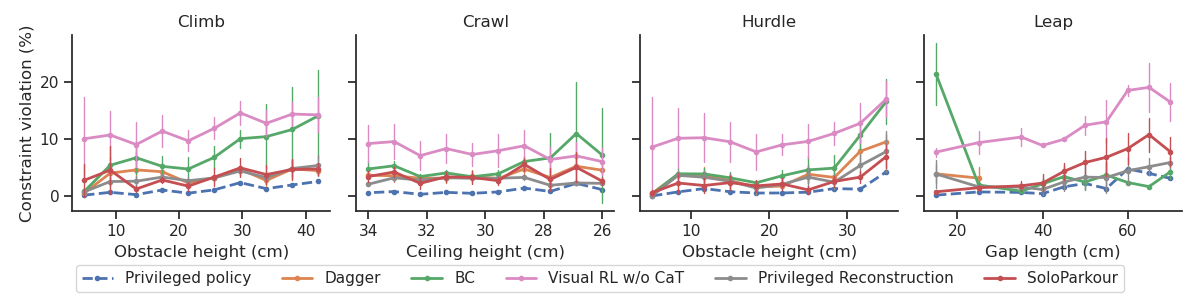
\includegraphics[width=\textwidth]{Assets/Results/base_ori_x0_exceeding.png}
        \caption{Constraint for the base orientation around the roll axis}
        \label{fig:torque1}
    \end{subfigure}

    \begin{subfigure}[b]{\textwidth}
        \centering
        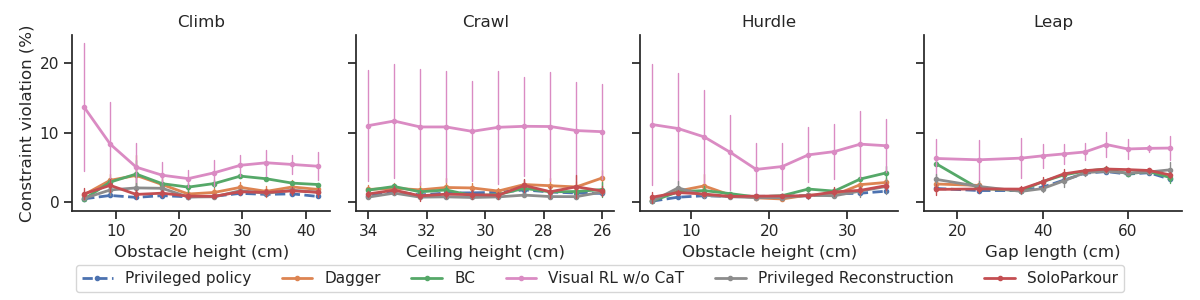
\includegraphics[width=\textwidth]{Assets/Results/torque2_exceeding.png}
        \caption{Torque constraint for the front left knee joint}
        
        \label{fig:torque2}
    \end{subfigure}
    \caption{Constraint violations (in \%) when the policies successfully traverse the terrain level by obstacle dimension, averaged across 4 training seeds.}
    \label{fig:torque_comparison}
    \vspace{-0.4cm}
\end{figure}